\subsection{Terminology}

% TODO: cite
According to Aho et al.  a \emph{compiler} is a program that
can read a program in one language --- the \emph{source} language --
and translates it into an equivalent program in another language --
the \emph{target} language; see Fig. \ref{fig:compiler}.

\begin{figure}[H]
  \centering
  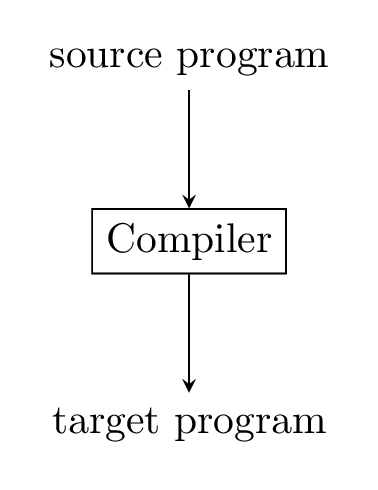
\includegraphics[width=0.3\textwidth]{figures/compiler.png}
  \caption{A compiler}
  \label{fig:compiler}
\end{figure}

Conversely, a \emph{decompiler} is also a that performs the reverse
operation of a compiler. It too, is a compiler. Commonly one views a
compiler as a translator from a high-level human-readable source
language into a low-level machine-readable language, similarly a
decompiler translates in the opposite direction; see
Fig. \ref{fig:decompiler}. 

The two exhibit a chiral relation to one another, i. e. that they are
mirrored images of each other in terms of functionality, but they are
not themselves identical.

\begin{figure}[H]
  \centering
  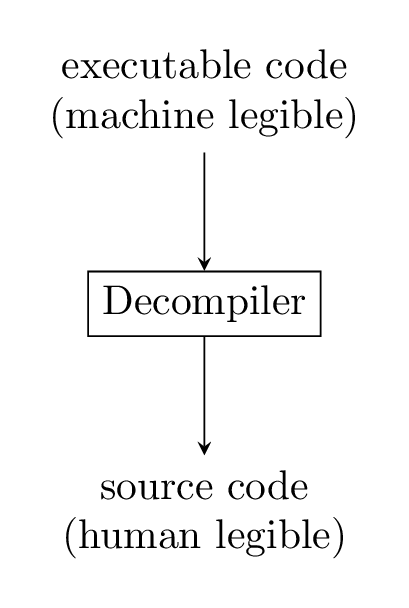
\includegraphics[width=0.3\textwidth]{figures/decompiler.png}
  \caption{A decompiler}
  \label{fig:decompiler}
\end{figure}

In this assignment the decompiler must be able to translate from the
machine-readable language of 32-bit numbers representing MIPS32
instructions to the human-readable target language described in the
introduction.

The constituent parts of the decompilers output will
be described further in section.~\ref{section:mul-example}.

Specifically,

\begin{itemize}
  \item Format.
  \item Opcode.
  \item Decomposed representation.
  \item Mnemonic representation.
\end{itemize}

will be covered. We will augment this list later on.
